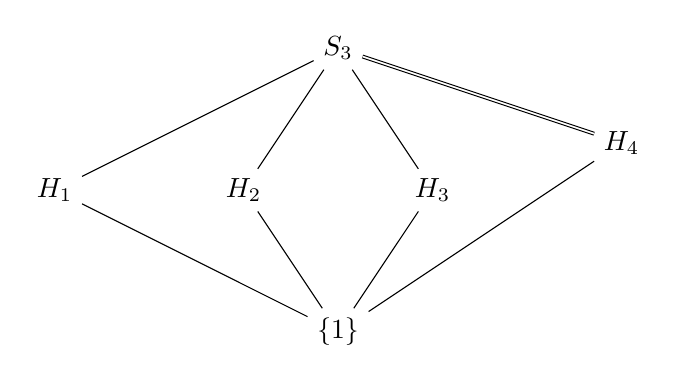
\begin{tikzpicture}[scale=1.2]
  % Nodes
  \node (S3) at (0,3) {$S_3$};

  \node (H1) at (-3,1.5) {$H_1$};
  \node (H2) at (-1,1.5) {$H_2$};
  \node (H3) at (1,1.5) {$H_3$};
  \node (H4) at (3,2) {$H_4$};

  \node (e) at (0,0) {$\{1\}$};

  % Edges from top
  \draw (S3) -- (H1);
  \draw (S3) -- (H2);
  \draw (S3) -- (H3);

  % Double line for normal subgroup
  \draw[double] (S3) -- (H4);

  % Edges to trivial subgroup
  \draw (H1) -- (e);
  \draw (H2) -- (e);
  \draw (H3) -- (e);

  % Double line again for normal chain
  \draw (H4) -- (e);
\end{tikzpicture}
